% 第 1 章 Working With the Fusion Compiler Tool
\bichapter{使用 Fusion Compiler 工具}{Working With the Fusion Compiler Tool}
\label{chap:fc}

Fusion Compiler 工具支持以下功能：
\begin{itemize}
  \item 提取（extraction）与时序分析（timing analysis）
  \item 物理综合与优化（physical synthesis and optimization）
  \item 布局与优化（含相对布局 relative placement）
  \item 时钟树综合（clock tree synthesis）
  \item 布线（routing）
  \item 芯片收尾（chip finishing）
  \item 层次化设计的顶层收敛（top-level closure）
  \item 工程变更指令（ECO）
  \item 报告（reporting）
  \item ASCII 输出接口
\end{itemize}

工具以 Verilog 网表、时序约束、逻辑与物理库以及晶圆厂工艺数据为输入；输出可为 OASIS 或 GDSII 格式的版图，或可供第三方路由器使用的已布局网表 DEF（Design Exchange Format）文件。也可随时将设计输出为二进制设计数据库，或以 ASCII 文件形式输出（Verilog、DEF 与时序约束）。

Fusion Compiler 还提供统一的：
\begin{itemize}
  \item \textbf{数据模型（data model）}：使库、设计数据、约束与设计意图可在整条实现流程中共享，并面向超大规模设计、以较小内存占用为目标进行架构；
  \item \textbf{图形用户界面（GUI）}：支持时序路径、功耗意图、原理图与版图的无缝可视化分析，并在 RTL 与网表之间提供完整交叉探测（cross-probing）；
  \item \textbf{设计不匹配缓解基础设施（design mismatch mitigation）}：提供用户可控手段，以应对不完整或不匹配的库与设计数据。
\end{itemize}

本章包括以下主题：
\begin{itemize}
  \item 物理综合设计流程概览
  \item 形式验证（Formal Verification）
  \item 布局布线设计流程概览
  \item Fusion Compiler 相关概念
  \item 使用 3DIC Compiler 用户界面
  \item 输入 \cmd{fc\_shell} 命令
  \item 使用应用选项（application options）
  \item 使用变量
  \item 查看 man 页
  \item 使用 Tcl 脚本
  \item 通过检查点（checkpoints）向脚本添加变更
  \item 使用 setup 文件
  \item 使用命令日志文件
  \item 启用多核处理
\end{itemize}

\begin{seeAlsoBox}
有关在 Fusion Compiler 中处理设计数据，请参阅 \textit{Fusion Compiler Data Model User Guide}。
\end{seeAlsoBox}

% ============================================================
\section{物理综合设计流程概览}
\subsection*{Physical Synthesis Design Flow Overview}

图~\ref{fig:physyn-flow} 给出基本的物理综合设计流程。

\begin{figure}[htbp]
\centering
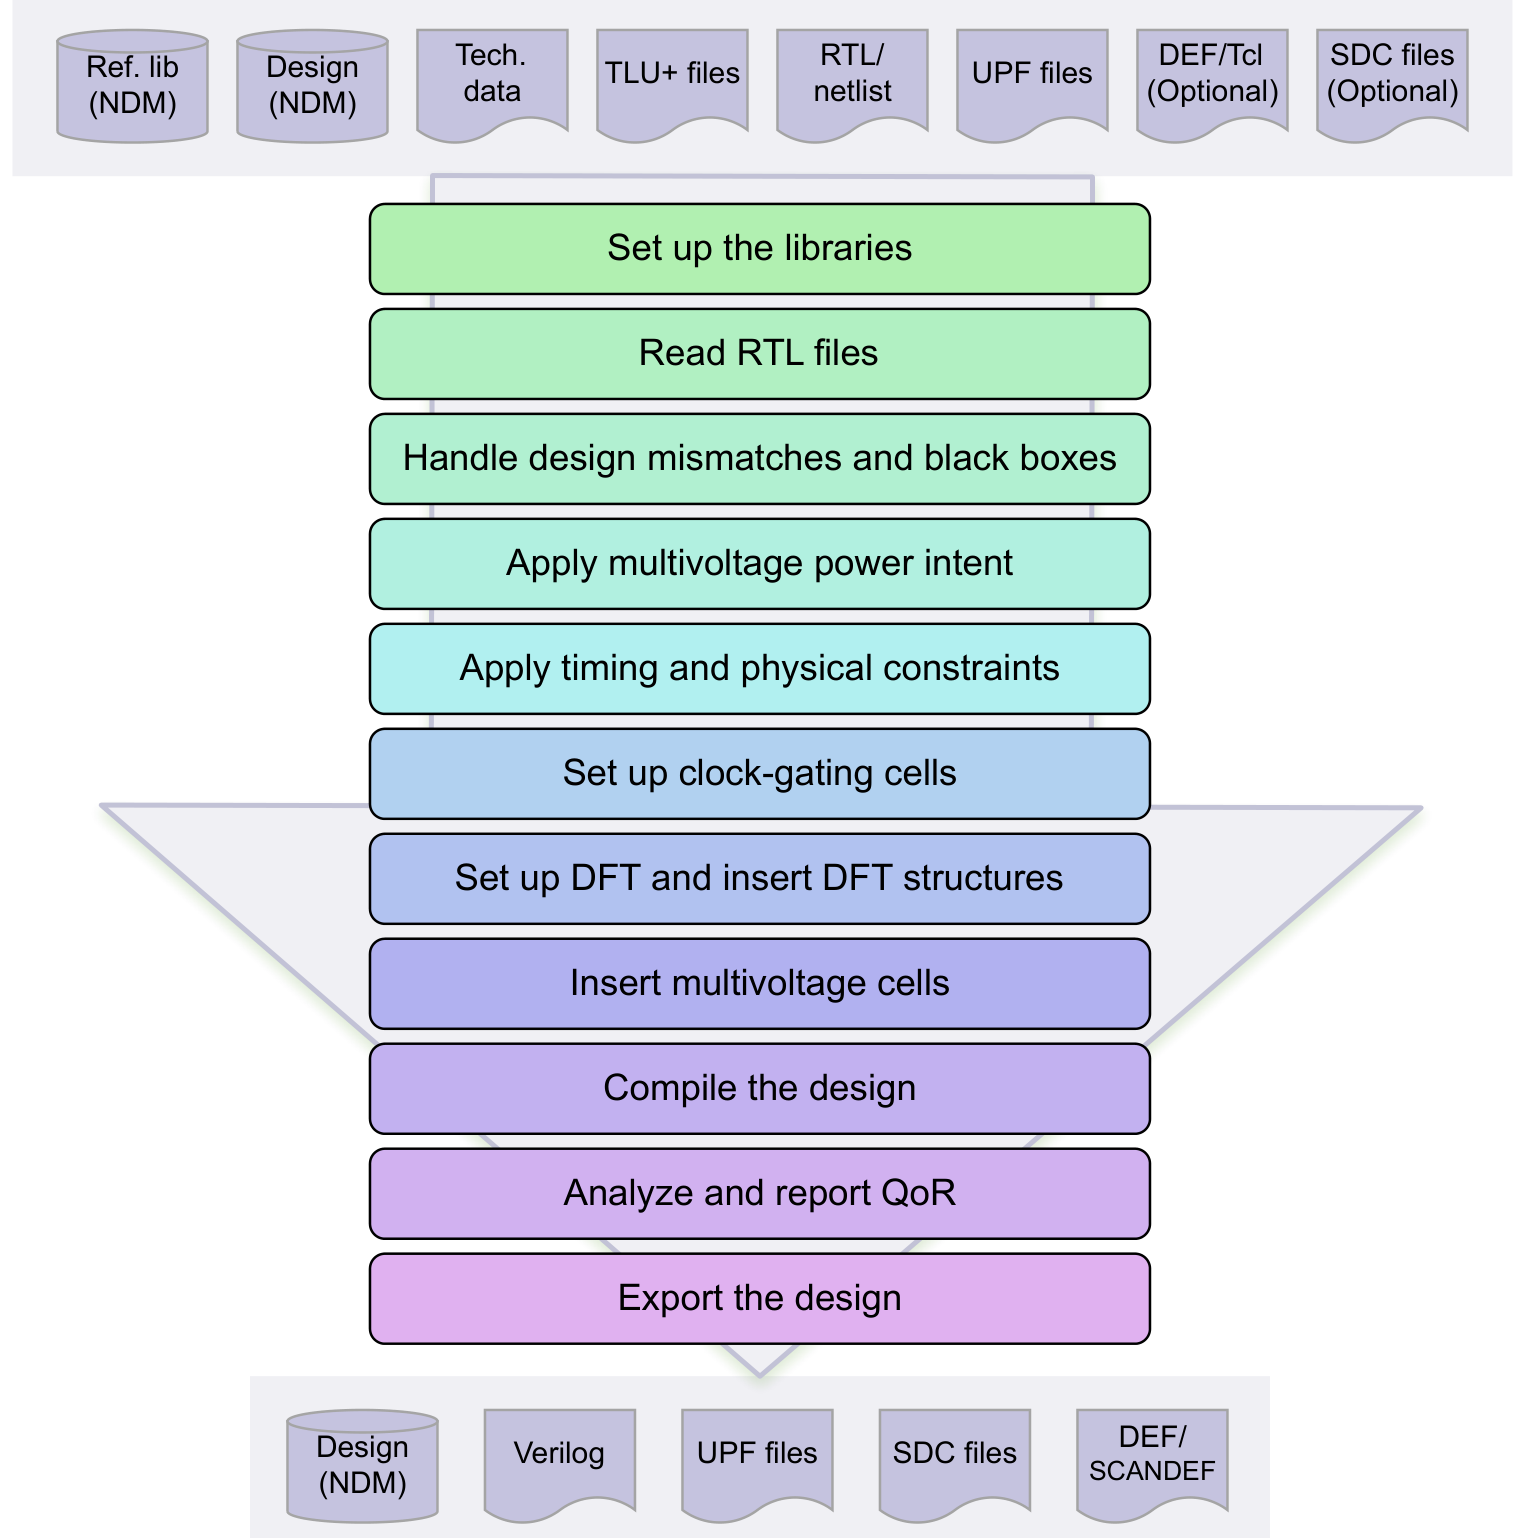
\includegraphics[width=0.85\textwidth,keepaspectratio]{figures/fig-physyn-flow.png}
\caption{Fusion Compiler 物理综合流程}
\label{fig:physyn-flow}
\end{figure}

% ============================================================
\section{形式验证}
\subsection*{Formal Verification}

Formality 工具使用形式化技术证明或否定两个设计的功能等价性，可执行 RTL-to-RTL、RTL-to-gate 与 gate-to-gate 验证。功能等价性检查不考虑静态时序验证。从 Fusion Compiler 到 Formality 的典型数据流包括：综合侧的 RTL/netlist、参考库（NDM）、工艺数据、TLU+、UPF、可选 DEF/Tcl、可选 SDC，以及 SVF 文件；再配合 Design（NDM）、Verilog、UPF 等输入 Formality。

\begin{figure}[htbp]
\centering
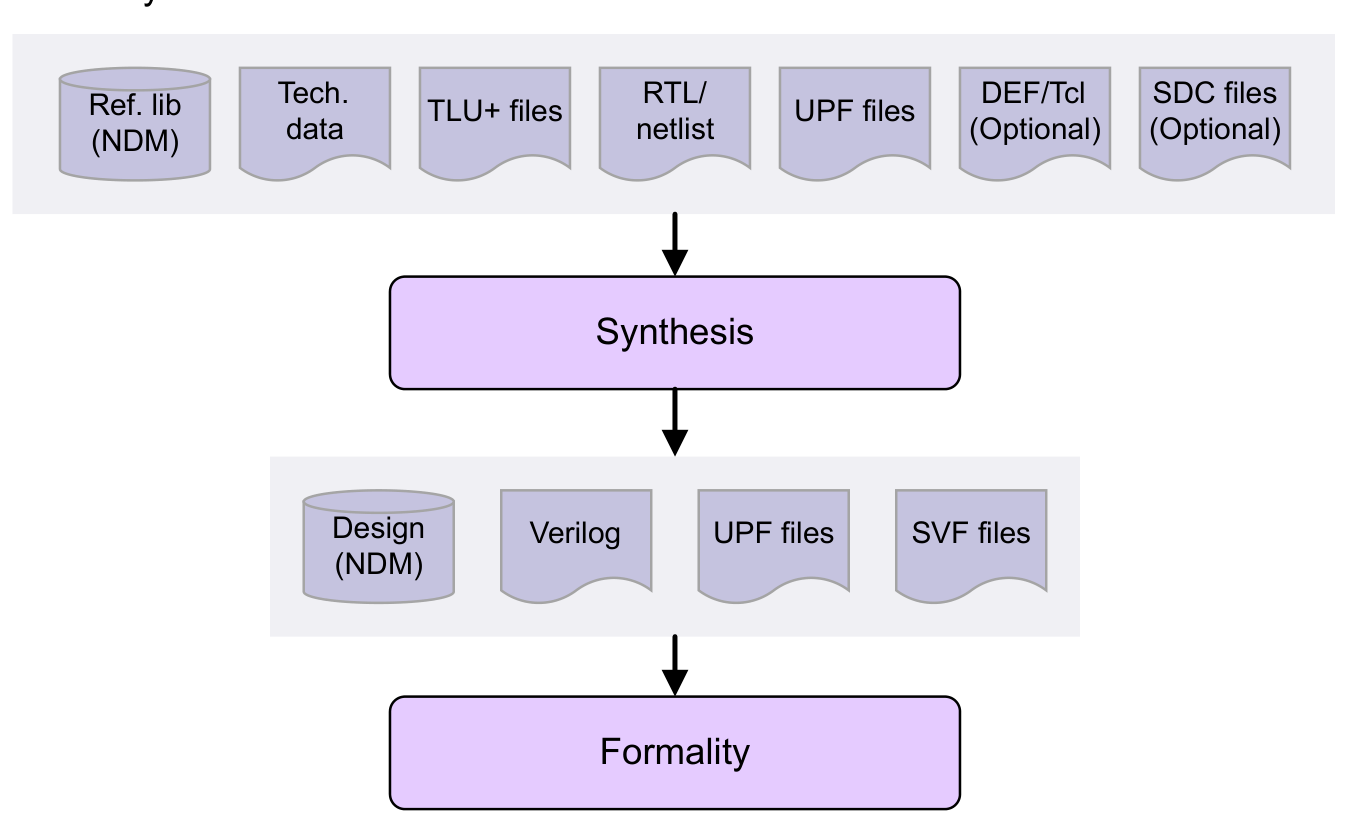
\includegraphics[width=0.85\textwidth,keepaspectratio]{figures/fig-formality-flow.png}
\caption{Fusion Compiler 到 Formality 的形式验证数据流}
\label{fig:formality-flow}
\end{figure}

% ============================================================
\section{布局布线设计流程概览}
\subsection*{Place and Route Design Flow Overview}

图~\ref{fig:pnr-flow} 给出使用 Fusion Compiler 的基本布局布线设计流程。

\begin{figure}[htbp]
\centering
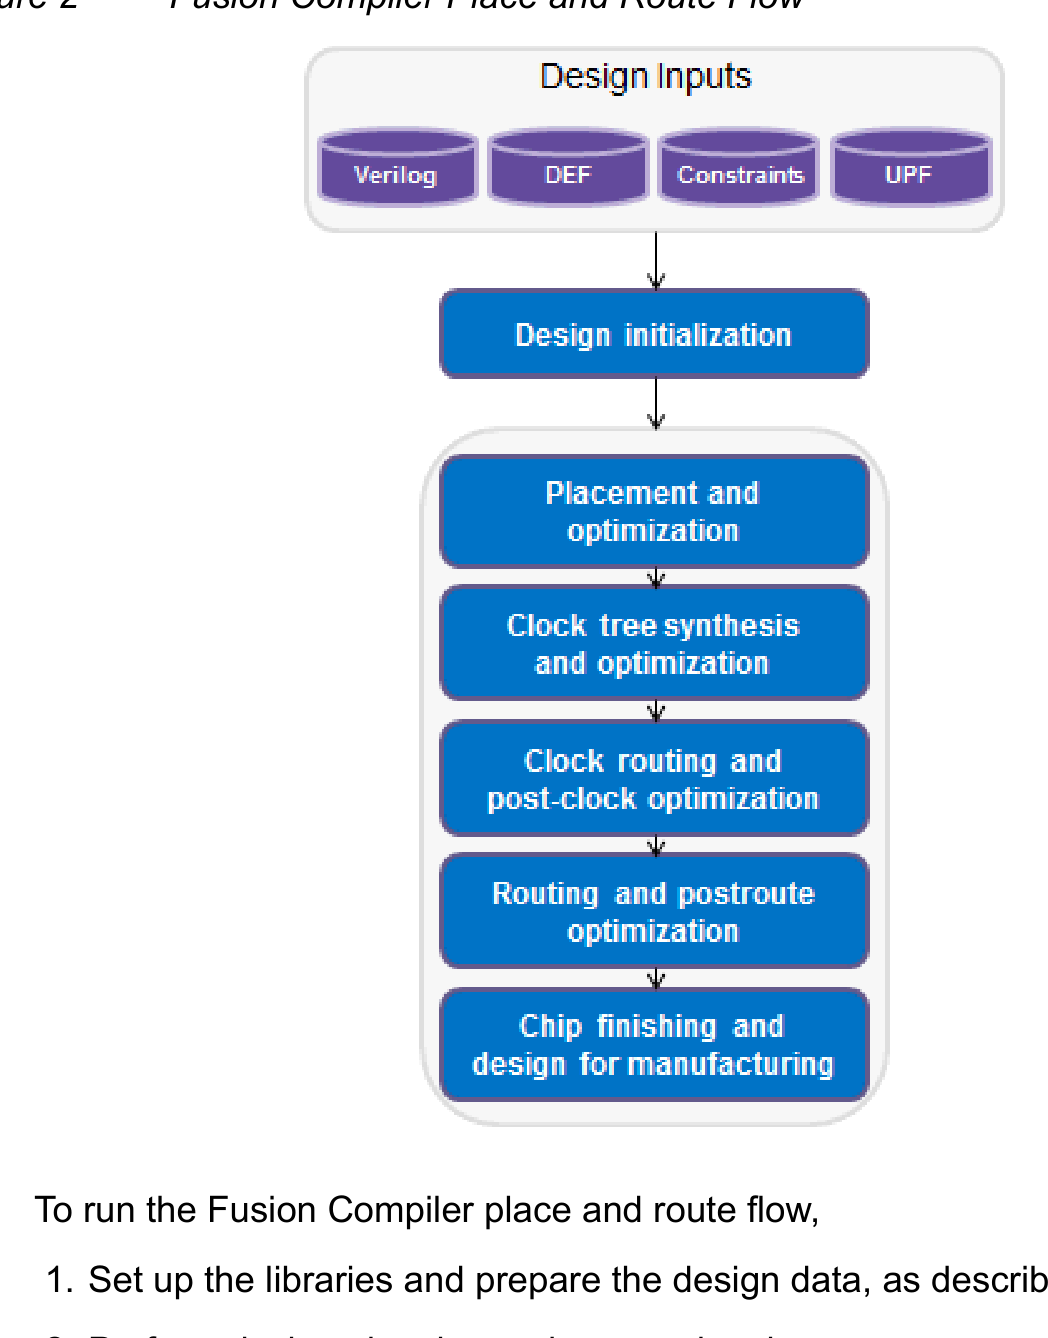
\includegraphics[width=0.55\textwidth,keepaspectratio]{figures/fig-pnr-flow.png}
\caption{Fusion Compiler 布局布线流程}
\label{fig:pnr-flow}
\end{figure}

运行 Fusion Compiler 布局布线流程的步骤如下：

\begin{enumerate}
  \item \textbf{设置库并准备设计数据}，见第~\ref{chap:prep}~章「准备设计」。
  \item \textbf{执行设计规划与电源规划}。\\
        此时创建 floorplan，以确定设计尺寸、创建边界与 core 区域、为标准单元布局创建 site rows、设置 I/O pad，并创建电源计划。\\
        更多信息见 \textit{Fusion Compiler Design Planning User Guide}。
  \item \textbf{执行布局与优化}。\\
        使用 \cmd{place\_opt} 命令。该命令面向并解决设计的时序收敛：通过增强的布局与综合技术，迭代生成叶单元（leaf cells）的合法化布局与优化后的设计。还可补充功耗优化、布局面积回收、降低拥塞，以及最小化时序与设计规则违例。
  \item \textbf{执行时钟树综合与优化}。\\
        使用 \cmd{clock\_opt} 命令。Fusion Compiler 的 CTS 与内嵌优化可处理复杂时钟树问题（如 blockage 规避、布线前与布线后数据相关性等）。时钟树优化通过缓冲器/门的尺寸调整与搬移、电平调整、重构、插入延时、插入 dummy load，以及平衡时钟间延时等方式，改善 skew 与 insertion delay。详见第~\ref{chap:cts}~章。
  \item \textbf{执行布线与布线后优化}，见第~\ref{chap:route}~章。\\
        工具使用 Zroute 进行全局布线、track assignment、详细布线、拓扑优化与 ECO 布线。布线后优化使用 \cmd{route\_opt}。对多数设计，默认设置即可；必要时可优化布线模式、降低串扰，或按特殊需求定制。
  \item \textbf{执行芯片收尾与可制造性设计（DFM）}，见第~\ref{chap:dfm}~章。\\
        可在流程各阶段应用芯片收尾、DFM 与可制造性（DFY）能力，以应对制造中的工艺设计问题。
  \item \textbf{保存设计}。
\end{enumerate}

% ============================================================
\section{Fusion Compiler 相关概念}
\subsection*{Fusion Compiler Concepts}

本节介绍工具中的以下概念：
\begin{itemize}
  \item 功耗意图（Power Intent）概念
  \item UPF 流程
  \item 多重图案化（Multiple-Patterning）概念
\end{itemize}

\subsection{功耗意图概念}
\subsubsection*{Power Intent Concepts}

UPF 语言定义了一组命令，用于规定电子系统的低功耗设计意图。通过 UPF，可描述供电网络、开关、隔离、保持（retention）以及与芯片功耗管理相关的其他方面。同一套低功耗规范应贯穿设计、分析、验证与实现流程。Synopsys 工具遵循正式的 IEEE 1801 UPF 标准。

UPF 规定设计的功耗需求，但不显式规定如何实现这些需求：它说明如何为各设计元素创建供电网络、供电网络之间的行为关系，以及如何扩展逻辑功能以支持对设计元素的动态电源开关；不包含布局或布线信息。

在 UPF 中，\textbf{power domain}（电源域）是逻辑层次中共享一组供电需求的元素集合。默认情况下，域内所有逻辑元素使用相同的主供电（primary supply）与主地（primary ground）；也可为域定义其他电源。电源域在物理版图上通常实现为连续的 voltage area，但这并非语言强制要求。

每个电源域有 \textbf{scope}（作用域）与 \textbf{extent}（范围）：scope 是被指定为该域根的逻辑层次；extent 是属于该域、共享相同供电需求的逻辑元素集合。scope 是定义域的层次，且是域内元素的祖先；extent 则是实际属于该域的元素集合。

每一 scope（层次）都有 \textbf{supply net}（供电网络）与 \textbf{supply port}（供电端口）。supply net 在给定电源域中承载供电电压或地；跨越多个电源域的 supply net 称为在多个域中「复用」。supply port 是相邻层次（父/子模块）之间的供电连接点；跨层次的 supply net 必须经过 supply port。

\textbf{Supply set}（供电网集合）是供电网络的抽象集合，包含 power 与 ground 两个供电功能。Supply set 与域无关：在创建该 supply set 的 scope 内，其 power 与 ground 可供任何电源域使用；但各电源域也可限制其对本域内 supply set 的使用。可在 RTL 级用 supply set 定义功耗意图，从而在尚不知实际 supply net 名称时即可综合设计。在物理实现（布局布线）之前，必须对 supply set 进行 refine（细化），即与实际 supply net 关联。

\textbf{Supply set handle} 是为电源域创建的抽象 supply set。默认情况下，电源域具有主供电、默认隔离供电与默认保持供电的 supply set handle。借助这些 handle，即使尚未为该域创建任何 supply set、supply net 与 supply port，也可综合设计。在物理实现前，须将 supply set handle refine 到实际 supply set，再将 supply set refine 到实际 supply net。

\textbf{Power switch}（电源开关）用于接通/关断某条 supply net 的供电，具有输入供电网、可开关的输出供电网，以及至少一个控制开关的输入信号；也可有多个控制输入与一个或多个应答输出。\textbf{Power state table} 列出设计中各电源域允许的电压值与开关状态组合。

当逻辑信号从一个电源域进入另一个电压明显不同的电源域时，必须插入 \textbf{level shifter}（电平移位单元）以转换摆幅。当逻辑信号离开可开关电源域并进入另一电源域时，必须插入 \textbf{isolation cell}（隔离单元），以便在关机期间产生确定逻辑值。若两域电压差异显著，接口单元需在上电时做电平移位、在关机时做隔离；能同时完成两者的单元称为 \textbf{enable level shifter}。

在具有电源开关的域中，关机期间需保持数据的寄存器必须实现为 \textbf{retention register}（保持寄存器），其具有独立的 always-on 供电（有时称 backup supply），在域主供电关闭时保持数据稳定。

\subsubsection{UPF 流程}
\subsubsection*{UPF Flows}

Fusion Compiler 同时支持传统 UPF 流程与 golden UPF 流程。Golden UPF 是维护多电压功耗意图的可选方法：在综合、物理实现与验证全过程中使用原始「golden」UPF 文件，并配合 Fusion Compiler 生成的 supplemental UPF 文件。

\begin{figure}[htbp]
\centering
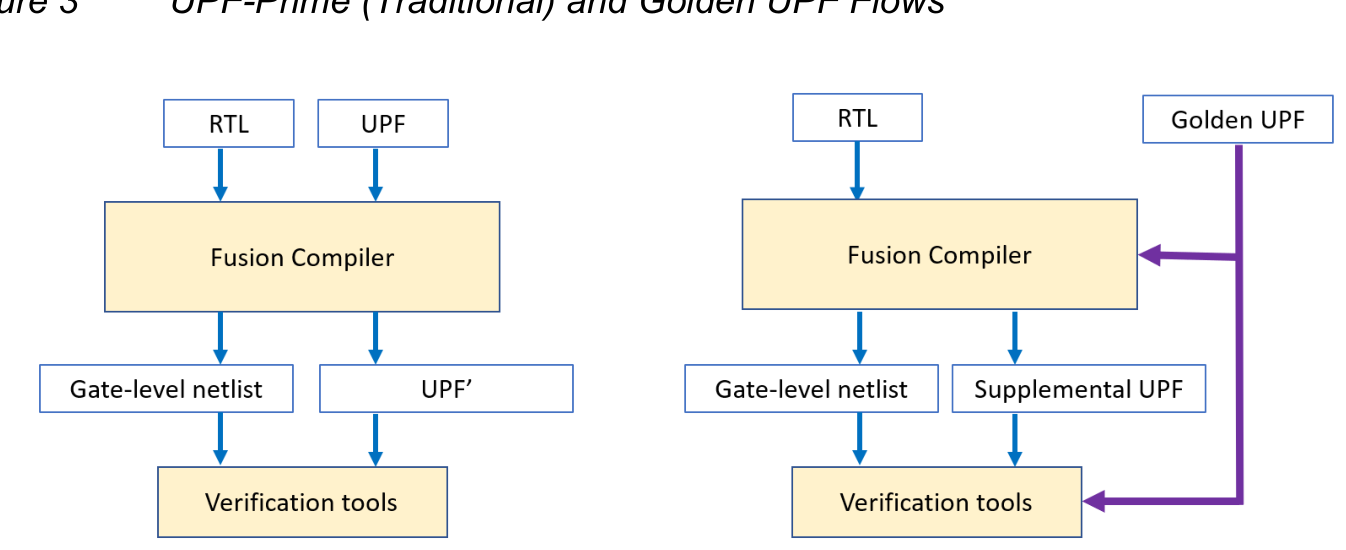
\includegraphics[width=0.92\textwidth,keepaspectratio]{figures/fig-upf-flows.png}
\caption{传统 UPF 与 Golden UPF 流程}
\label{fig:upf-flows}
\end{figure}

Golden UPF 流程在整条链路中保持并使用同一份原始 golden UPF；工具将功耗意图变更写入单独的 supplemental UPF。下游与验证工具使用 golden + supplemental 的组合，而不是单一的 UPF' 或 UPF'' 文件。

其优势包括：
\begin{itemize}
  \item golden UPF 在流程中保持不变，保留原始结构、注释与通配命名；
  \item 可使用工具相关条件语句在不同工具中执行不同任务（传统 UPF-prime 流程中会丢失）；
  \item 功耗意图变更易于在 supplemental 文件中追踪；
  \item 可选地用 Verilog 网表存储全部 PG 连接信息，从而不必在 UPF 中使用 \cmd{connect\_supply\_net}，显著简化并缩小 UPF。
\end{itemize}

在加载 UPF 之前，用下列应用选项启用 golden UPF 流程：
\begin{lstlisting}
fc_shell> set_app_options -as_user_default \
   -list {mv.upf.enable_golden_upf true}
\end{lstlisting}

加载 supplemental UPF 时，对 \cmd{load\_upf} 使用 \opt{-supplemental} 选项。更多信息见 SolvNet 文章 1412864，\textit{Golden UPF Flow Application Note}。

\subsection{多重图案化概念}
\subsubsection*{Multiple-Patterning Concepts}

在 20~nm 及以下工艺节点，现有光刻工具难以印制所需几何图形。为此采用 \textbf{多重图案化}：将版图掩模划分为两张或更多掩模，以提高制造间距、分辨率与可印制性。图~\ref{fig:dp-example} 给出双图案化示例（MASK A / MASK B）。

\begin{figure}[htbp]
\centering
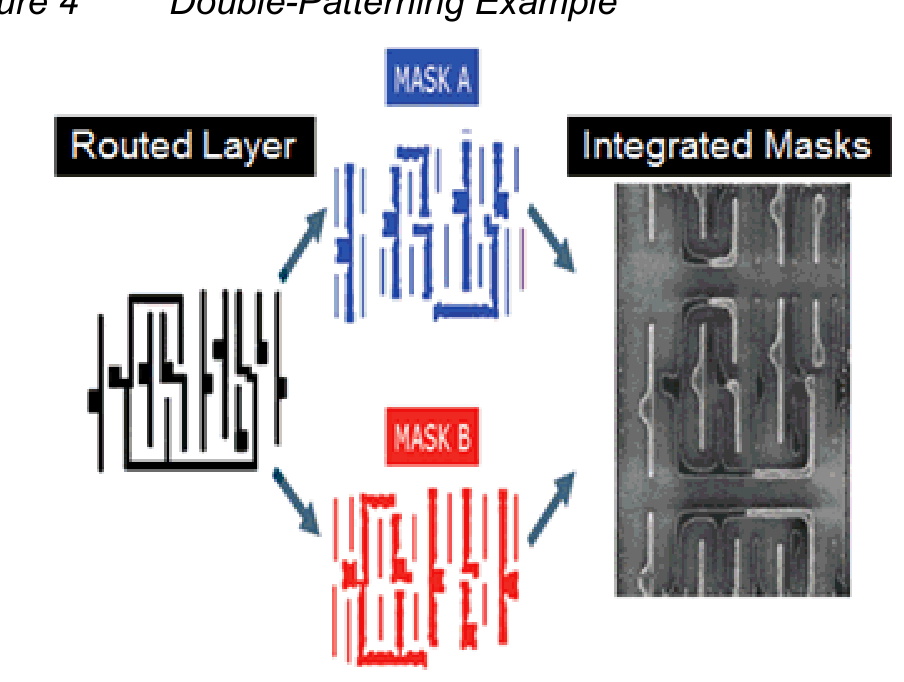
\includegraphics[width=0.92\textwidth,keepaspectratio]{figures/fig-dp-example.png}
\caption{双图案化示例}
\label{fig:dp-example}
\end{figure}

使用多重图案化时，必须能将版图分解为满足多重图案化间距要求的两张或多张掩模。若某区域中相邻图形对数为奇数，且每对间距均小于多重图案化最小间距，则出现违例，称为 \textbf{odd cycle}（奇环），见图~\ref{fig:odd-cycle}。

\begin{figure}[htbp]
\centering
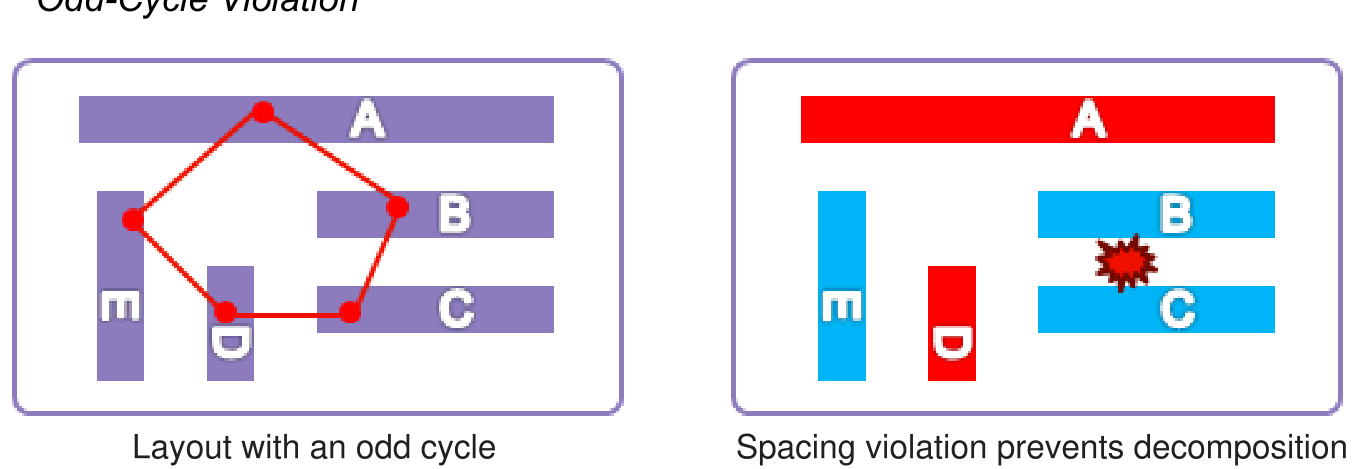
\includegraphics[width=0.92\textwidth,keepaspectratio]{figures/fig-odd-cycle.png}
\caption{奇环违例}
\label{fig:odd-cycle}
\end{figure}

若环中任一对间距大于多重图案化最小间距，则无违例，版图可分解（例如图~\ref{fig:no-odd-cycle} 中 B 与 C 间距 $x$ 足够大）。

\begin{figure}[htbp]
\centering
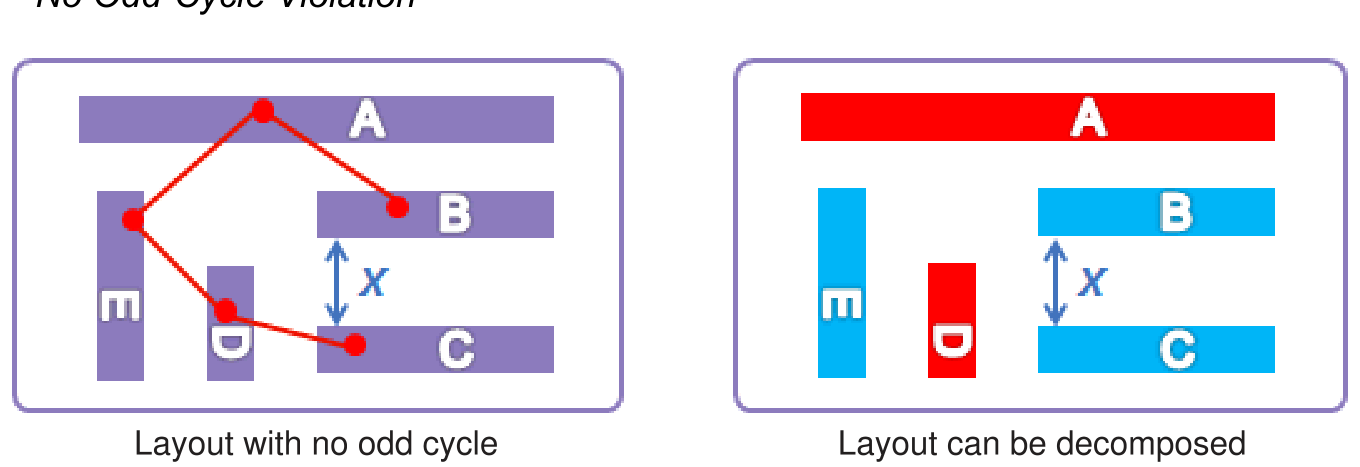
\includegraphics[width=0.92\textwidth,keepaspectratio]{figures/fig-no-odd-cycle.png}
\caption{无奇环违例}
\label{fig:no-odd-cycle}
\end{figure}

Fusion Compiler 在布局与布线中考虑多重图案化间距要求并防止奇环，使版图利于双图案化。一般仅在最底层金属（multiple-patterning layers）上执行双图案化；这些层上的金属形状（无论布线还是标准单元/宏内金属）须满足更严格间距；其他层不必。

多重图案化影响布局布线全流程。根据标准单元库，可走 \textbf{uncolored} 或 \textbf{precolored} 流程：
\begin{itemize}
  \item \textbf{Uncolored 流程}：单元到边界有足够间距，布局时不会产生多重图案化违例。此类库称 correct-by-construction library（多数多重图案化库属此类）。工具为 pin 与 net shape 决定合适的 mask 设置。
  \item \textbf{Precolored 流程}：单元内部金属形状已分配 mask（常称 color），此类库称 precolored library。工具必须考虑这些分配，避免布局违例，并据此决定 pin/net 的 mask。Mask 分配在工具中表现为 \textbf{mask constraints}，须在开始布局布线前正确设置。
\end{itemize}

\subsubsection{掩模约束}
\subsubsection*{Mask Constraints}

Mask constraints 表示采用多重图案化技术的 block 中物理 pin 与 net 金属形状的掩模要求，驱动布局与布线以保证版图合规。

\begin{noteBox}
Mask constraints 仅用于 precolored 流程；uncolored 流程不需要。
\end{noteBox}

可对时序关键 net（net shapes、routing rules、routing blockages）以及 via 设置 mask constraints。对 net，约束定义在 \appopt{mask\_constraint} 属性；对 via，定义在 \appopt{lower\_mask}、\appopt{upper\_mask}、\appopt{cut\_mask}。支持取值见表~\ref{tab:mask}。

\begin{table}[htbp]
\centering
\caption{Mask Constraint 取值}
\label{tab:mask}
\begin{tabularx}{\textwidth}{@{}l X@{}}
\toprule
\textbf{属性值} & \textbf{说明} \\
\midrule
\cmd{same\_mask} & 掩模颜色尚未确定。带此属性的形状与任意已着色金属形状之间至少须满足多重图案化最小间距。 \\
\cmd{mask\_one} & 形状为 mask1 色；与其他 mask1 形状之间至少须满足多重图案化最小间距。 \\
\cmd{mask\_two} & 形状为 mask2 色；与其他 mask2 形状之间至少须满足多重图案化最小间距。 \\
\cmd{mask\_three} & 形状为 mask3 色；与其他 mask3 形状之间至少须满足多重图案化最小间距。 \\
\cmd{any\_mask} & 形状未着色；仅需满足标准最小间距，多重图案化最小间距规则不适用。 \\
\bottomrule
\end{tabularx}
\end{table}

% ============================================================
\section{使用 3DIC Compiler 用户界面}
\subsection*{Working With the 3DIC Compiler User Interfaces}

Fusion Compiler 在 Linux 上的 X Window 环境中运行，同时提供 shell 命令行界面（CLI）与 GUI。会话期间 CLI 始终可用；可在 shell 或 GUI 中启动/退出会话，也可在会话中打开或关闭 GUI。

工具使用 Tcl（EDA 业界广泛采用）。可用 Tcl 通过可复用过程与脚本扩展 \cmd{fc\_shell} 命令语言（见 \textit{Using Tcl With Synopsys Tools}）。

本节说明如何用命令行启动与退出工具：
\begin{itemize}
  \item 启动 CLI
  \item 退出 Fusion Compiler
\end{itemize}
GUI 用法见 \textit{Fusion Compiler Graphical User Interface User Guide}。另见：启动 GUI、关闭 GUI。

\subsection{启动 CLI}
\subsubsection*{Starting the CLI}

CLI 是纯文本环境，在提示符下输入命令，常用于脚本、批处理与一键流程。启动前请确保 \texttt{bin} 目录已在 \texttt{\$PATH} 中。

启动方式：在 Linux shell 中输入
\begin{lstlisting}
% fc_shell
\end{lstlisting}

启动时可附加选项，例如：
\begin{itemize}
  \item \opt{-file script\_file\_name}：执行脚本
  \item \opt{-x command}：执行一条命令
  \item \opt{-output\_log\_file file\_name}：创建会话日志
  \item \opt{-help}：列出可用选项（不启动 shell）
\end{itemize}

启动时工具依次：
\begin{enumerate}
  \item 创建命令日志文件；
  \item 读取并执行 setup 文件；
  \item 执行命令行 \opt{-file}/\opt{-x} 指定的脚本或命令；
  \item 显示程序头与 \cmd{fc\_shell>} 提示符。
\end{enumerate}

\begin{seeAlsoBox}
使用命令日志文件；使用 setup 文件；使用 Tcl 脚本。
\end{seeAlsoBox}

\subsection{退出工具}
\subsubsection*{Exiting the Fusion Compiler Tool}

可用 \cmd{exit} 或 \cmd{quit} 随时结束会话。

\begin{noteBox}
从命令行退出时，工具\textbf{不会}保存已打开的 block。
\end{noteBox}

% ============================================================
\section{输入 fc\_shell 命令}
\subsection*{Entering fc\_shell Commands}

与工具交互使用基于 Tcl 并带有 Fusion Compiler 扩展的 \cmd{fc\_shell} 命令。命令语言提供类似 Linux shell 的变量、条件执行与流程控制。你可以：
\begin{itemize}
  \item 在 \cmd{fc\_shell>} 提示符下交互输入；
  \item 在 GUI 控制台命令行交互输入；
  \item 运行包含 \cmd{fc\_shell} 命令的 Tcl 脚本。
\end{itemize}

输入命令、选项或文件名时，可在字符足以唯一确定名称后按 Tab 自动补全；若有多个候选，工具会列出并由方向键与 Enter 选择。

若需复用命令行输出中的内容，可选中后移到命令行并用鼠标中键粘贴。

运行命令时，输出（含处理信息、警告与错误）会回显到 \cmd{fc\_shell}；若 GUI 打开，也会出现在控制台日志视图。默认非分页模式，输出可能滚动。要启用分页，将 \cmd{sh\_enable\_page\_mode} 设为 \cmd{true}。

\subsection{中断或终止命令处理}
\subsubsection*{Interrupting or Terminating Command Processing}

若选项或命令有误，可中断处理并留在 \cmd{fc\_shell} 中：按 \textbf{Ctrl+C}。

某些命令/进程不可中断，须在系统级终止 \cmd{fc\_shell}；终止进程或 shell 时\textbf{不保存}任何数据。

使用 Ctrl+C 时注意：
\begin{itemize}
  \item 若正在处理脚本且中断其中一条命令，脚本处理被中断，后续脚本命令不再执行；
  \item 若在命令响应中断前连续按三次 Ctrl+C，\cmd{fc\_shell} 会被中断并以如下信息退出：\\
        \texttt{Information: Process terminated by interrupt.}
\end{itemize}

\subsection{获取命令信息}
\subsubsection*{Getting Information About Commands}

在线资源包括：
\begin{itemize}
  \item 命令帮助（command help）
  \item Man pages
\end{itemize}

\subsubsection{显示命令帮助}
\subsubsection*{Displaying Command Help}

命令帮助可以是命令的简要说明，或其所支持选项与参数的列表。
\begin{itemize}
  \item 简要说明：\cmd{help} 后跟命令名，例如
\begin{lstlisting}
fc_shell> help report_timing
\end{lstlisting}
  \item 选项列表：命令名加 \opt{-help}，例如
\begin{lstlisting}
fc_shell> report_timing -help
\end{lstlisting}
\end{itemize}

% ============================================================
\section{使用应用选项}
\subsection*{Using Application Options}

应用选项（application options）控制工具行为，命名约定为：
\begin{center}
\cmd{category[.subcategory].option\_name}
\end{center}
其中 \cmd{category} 为受影响引擎名；部分类别还有子类别。

作用域分为：
\begin{itemize}
  \item \textbf{Block 作用域}：仅作用于设置所在的 block，保存在设计库中，跨会话持久。
  \item \textbf{Global 作用域}：作用于所有 block，但仅在当前会话有效，不写入设计库；每个 \cmd{fc\_shell} 会话都需重新指定。可将全局设置加入 \texttt{.synopsys\_fc.setup}。
\end{itemize}

列出可用应用选项：\cmd{get\_app\_options}（默认可列出全部；可提供 pattern 限制）。
\begin{lstlisting}
fc_shell> get_app_options
fc_shell> get_app_options timer.*
\end{lstlisting}

生成报告：\cmd{report\_app\_options}。详细说明见 \textit{Fusion Compiler Data Model User Guide} 中的 Application Options。

\begin{seeAlsoBox}
使用 setup 文件。
\end{seeAlsoBox}

% ============================================================
\section{使用变量}
\subsection*{Using Variables}

一般而言，Fusion Compiler 通过应用选项而非应用变量修改默认行为；但仍支持用户定义的 Tcl 变量，以及少量应用变量（如 \cmd{search\_path}）。

列出变量及其值：\cmd{printvar}。
\begin{lstlisting}
fc_shell> printvar *
fc_shell> printvar search_path
\end{lstlisting}

\begin{seeAlsoBox}
定义搜索路径（Defining the Search Path）。
\end{seeAlsoBox}

% ============================================================
\section{查看 Man 页}
\subsection*{Viewing Man Pages}

显示命令或应用选项的 man 页：\cmd{man} 后跟名称。例如：
\begin{lstlisting}
fc_shell> man report_timing
\end{lstlisting}

也可查看应用选项摘要页：
\begin{itemize}
  \item \textbf{类别摘要}：\cmd{man category\_options}，例如
\begin{lstlisting}
fc_shell> man timer_options
\end{lstlisting}
  \item \textbf{子类别摘要}：\cmd{man category.subcategory\_options}，例如
\begin{lstlisting}
fc_shell> man route.common_options
\end{lstlisting}
  \item \textbf{命令相关摘要}：\cmd{man command\_options}，例如
\begin{lstlisting}
fc_shell> man report_timing_options
\end{lstlisting}
\end{itemize}

在 \cmd{fc\_shell} 中输入 \cmd{man} 时，man 页显示在 shell 中（GUI 打开时亦在控制台日志）；在 GUI 控制台输入时，显示在 GUI man 页查看器中。

% ============================================================
\section{使用 Tcl 脚本}
\subsection*{Using Tcl Scripts}

可用 Tcl 脚本完成例行、重复或复杂任务：将 Fusion Compiler 命令序列放入文本文件即可；任何 Fusion Compiler 命令都可在脚本中执行。

Tcl 中以 \texttt{\#} 开头的行为注释，例如：
\begin{lstlisting}
# This is a comment
\end{lstlisting}

编写脚本详见 \textit{Using Tcl With Synopsys Tools}。运行脚本的方式：
\begin{itemize}
  \item 启动时使用 \cmd{fc\_shell -file}；
  \item 在命令行使用 \cmd{source}；
  \item GUI 中选择 File $>$ Execute Script。
\end{itemize}

命令出错时工具会抛出 \cmd{TCL\_ERROR} 并立即停止脚本。若要容忍错误并继续执行，可：
\begin{itemize}
  \item 对可能出错的命令用 Tcl \cmd{catch} 检查 \cmd{TCL\_ERROR}；
  \item 或在脚本中将 \cmd{sh\_continue\_on\_error} 设为 \cmd{true}。
\end{itemize}

\begin{seeAlsoBox}
启动 CLI；通过检查点向脚本添加变更。
\end{seeAlsoBox}

% ============================================================
\section{通过检查点向脚本添加变更}
\subsection*{Adding Changes to a Script With Checkpoints}

在 block 上做实验时，可能以两种方式修改 golden flow 脚本：
\begin{itemize}
  \item 流程变更：设置应用选项、修改约束或其他改进 QoR 的改动；
  \item 生成报告：增加报告或在流程新位置报告，便于调试。
\end{itemize}

多数流程通过少量静态可改文件施加变更。典型 \cmd{place\_opt} 流程示例：source \texttt{pre\_place\_opt\_settings.tcl} 做流程改动，末尾 source \texttt{generate\_reports.tcl} 统一报告：
\begin{lstlisting}
open_block ./design:init_design
source ./scripts/pre_place_opt_settings.tcl
remove_buffer_trees -all
place_opt -from initial_place -to initial_drc
create_placement -incremental -timing_driven -congestion
place_opt -from initial_drc -to initial_opto
place_opt -from final_place -to final_opto
source ./scripts/generate_reports.tcl
\end{lstlisting}

复杂改动有时需要直接改 golden 脚本，这在许多设计环境中不被鼓励或很难做，尤其当需在多阶段、多 block 或多组实验中实施时。

\textbf{检查点（checkpoint）系统}可简化该过程，使你无需修改 golden flow 脚本即可实验：在 golden flow 的重要步骤处定义 checkpoint，包裹相关命令。默认仅运行所包裹代码——单纯插入 checkpoint \textbf{不会}改变流程。但可将 checkpoint 与「在包裹代码之前 / 之后 / 替代」执行的流程变更或报告关联；这些关联定义在可移植配置文件中，从而把 golden 脚本与某次运行的变更隔离。

同一配置文件可复制到各设计的 run 目录，从而在不修改各设计 golden 脚本的情况下统一施加变更。多用户项目中，每人可有独立的 \texttt{checkpoint.config.tcl}。

检查点系统还支持：
\begin{itemize}
  \item 比非 checkpoint 脚本更精确地插入流程变更与报告；
  \item 以单一真相来源查看对默认 golden flow 的全部变更；
  \item 报告已运行 checkpoint 的历史，含当时执行的变更/报告；
  \item 报告各 checkpoint 的 runtime 与 memory；
  \item 生成唯一且描述性的报告名。
\end{itemize}

一般步骤：
\begin{enumerate}
  \item 在脚本中插入 checkpoints；
  \item 配置：定义要关联的流程变更/报告，并与 checkpoints 关联；
  \item 运行脚本。
\end{enumerate}

\subsection{定义检查点}
\subsubsection*{Defining Checkpoints}

使用 \cmd{eval\_checkpoint}，指定唯一名称并包裹代码块。

注意：
\begin{itemize}
  \item 若新定义名称与已有 checkpoint 重名，运行遇到时工具会自动加唯一后缀（如 \cmd{placement} $\rightarrow$ \cmd{placement2}）；
  \item 不要嵌套 checkpoint：工具虽不阻止定义，但运行时忽略嵌套 checkpoint，只执行最外层（嵌套内的 Tcl 仍会执行，只是仿佛没有 checkpoint）。
\end{itemize}

示例：为 golden flow 各主要步骤包裹 checkpoint：
\begin{lstlisting}
open_block ./design.nlib:init_design
source ./scripts/pre_place_opt_settings.tcl

eval_checkpoint remove_buffers {
    remove_buffer_trees -all
}

eval_checkpoint place_opt_to_initial_drc {
    place_opt -from initial_place -to initial_drc
}

eval_checkpoint incr_placement {
    create_placement -incremental -timing_driven -congestion
}

eval_checkpoint place_opt_to_initial_opto {
    place_opt -from initial_drc -to initial_opto
}

eval_checkpoint place_opt_to_final_opto {
    place_opt -from final_place -to final_opto
}
\end{lstlisting}

默认仅运行包裹代码；关联行为见下一小节。

\subsection{配置检查点}
\subsubsection*{Configuring Checkpoints}

要使 checkpoint 影响流程，须将其与「之前 / 之后 / 替代」执行的流程变更或报告关联。

\subsubsection{定义检查点行为}
\subsubsection*{Defining Checkpoint Behaviors}

可定义两类行为：\textbf{reports} 与 \textbf{actions}。Report 用于生成工具支持的报告或自定义报告；Action 用于在 checkpoint 包裹代码之前、之后或替代执行任意流程变更（例如在某 checkpoint 前设置应用选项）。

这些行为定义在检查点系统自动 source 的 \texttt{checkpoint.config.tcl} 中。

\paragraph{定义 Checkpoint Reports}
使用 \cmd{create\_checkpoint\_report}，指定唯一名称与生成报告的 Tcl：
\begin{lstlisting}
create_checkpoint_report timing {
   set name [get_current_checkpoint -name]
   set pos  [get_current_checkpoint -position]

    report_qor -nosplit > ./checkpoint/$name.$pos.qor.rpt
    report_qor -summary -nosplit >> ./checkpoint/$name.$pos.qor.rpt

    report_timing -nosplit -max_paths 10 \
       > ./checkpoint/$name.$pos.path.rpt
}
\end{lstlisting}

注意用 \cmd{get\_current\_checkpoint -name/-position} 为报告命名：触发的 checkpoint 名以及 before/after 位置会体现在文件名中（例如 \texttt{checkpoint\_A.after.qor.rpt}）。

再如写出全部非默认应用选项：
\begin{lstlisting}
create_checkpoint_report app_options {
   set name [get_current_checkpoint -name]
   set pos  [get_current_checkpoint -position]
    report_app_options -non_default \
       > ./checkpoint/$name.$pos.app_options.rpt
}
\end{lstlisting}

\paragraph{定义 Checkpoint Actions}
使用 \cmd{create\_checkpoint\_action}。例如启用基于全局布线的 buffering：
\begin{lstlisting}
create_checkpoint_action gropto {
   set_app_options -name place_opt.initial_drc.global_route_based \
      -value true
}
\end{lstlisting}

高努力拥塞缓解示例（用 \cmd{get\_current\_checkpoint -script} 取回原包裹命令并追加选项）：
\begin{lstlisting}
create_checkpoint_action placer_high_effort_cong {
      set placer_command [get_current_checkpoint -script]
      set cong_option "-congestion_effort high"
      eval $placer_command $cong_option
}
\end{lstlisting}

\subsubsection{关联检查点与行为}
\subsubsection*{Associating Checkpoints and Checkpoint Behaviors}

定义 checkpoint 与 behavior 后，须用关联命令使运行遇到 checkpoint 时执行行为。

\paragraph{关联 Reports}
使用 \cmd{associate\_checkpoint\_report}：
\begin{itemize}
  \item \opt{-enable}：报告名；
  \item \opt{-before} / \opt{-after}：在指定 checkpoint 之前/之后运行；
  \item 多个 checkpoint 可列名或用 \texttt{*} 通配。
\end{itemize}

示例：
\begin{lstlisting}
associate_checkpoint_report -enable timing \
   -after { place_opt_to_initial_opto place_opt_to_final_opto }

associate_checkpoint_report -enable app_options -before *
\end{lstlisting}

\paragraph{关联 Actions}
使用 \cmd{associate\_checkpoint\_action}：
\begin{itemize}
  \item \opt{-enable}：action 名；
  \item \opt{-before} / \opt{-after} / \opt{-replace}：之前、之后或\textbf{替代}包裹代码。
\end{itemize}

示例：
\begin{lstlisting}
associate_checkpoint_action -enable gropto \
   -before place_opt_to_initial_drc

associate_checkpoint_action -enable placer_high_effort_cong \
   -replace incr_placement
\end{lstlisting}

\paragraph{同一 Checkpoint 关联多个行为时的执行顺序}
\begin{enumerate}
  \item 配置为 before 的 reports；
  \item 配置为 before 的 actions；
  \item checkpoint 包裹代码，或配置为 replace 的 actions；
  \item 配置为 after 的 actions；
  \item 配置为 after 的 reports。
\end{enumerate}
同一位置有多个 report/action 时，按 \cmd{associate\_checkpoint\_*} 关联的先后顺序执行。

\subsection{查询检查点与行为}
\subsubsection*{Querying Checkpoints and Checkpoint Behaviors}

使用 \cmd{get\_checkpoint\_data}：
\begin{lstlisting}
fc_shell> get_checkpoint_data -list_names
fc_shell> get_checkpoint_data -name place_opt_to_initial_drc
fc_shell> get_checkpoint_data -list_reports
fc_shell> get_checkpoint_data -list_actions
fc_shell> get_checkpoint_data -report app_options
\end{lstlisting}

\subsection{查看检查点历史}
\subsubsection*{Viewing Your Checkpoint History}

进入 \texttt{checkpoint} 目录：其中 \texttt{checkpoint\_history.rpt} 记录每次运行遇到的 checkpoint 及 runtime/memory；该目录也存放写出的 checkpoint reports。

清除历史：
\begin{itemize}
  \item \cmd{reset\_checkpoints}：清空整个 checkpoint 目录（含报告）；清空前会在 run 目录保存带时间戳的副本；
  \item \cmd{reset\_checkpoints -from <name>}：从指定 checkpoint 起（含）从历史中移除后续条目，但\textbf{不}删除已写出的报告文件。
\end{itemize}

% ============================================================
\section{使用 Setup 文件}
\subsection*{Using Setup Files}

启动时工具自动执行 \texttt{.synopsys\_fc.setup} 中的命令。会在家目录与项目目录（启动时的当前工作目录）中查找，读取顺序为：
\begin{enumerate}
  \item 家目录中的 \texttt{.synopsys\_fc.setup}
  \item 项目目录中的 \texttt{.synopsys\_fc.setup}
\end{enumerate}

Setup 文件可包含初始化应用选项、设置 GUI 选项等基本任务。例如：
\begin{itemize}
  \item 在家目录 setup 中设置定义工作环境的应用选项；
  \item 在设计目录 setup 中设置影响某 block 处理的项目/block 专用选项。
\end{itemize}

% ============================================================
\section{使用命令日志文件}
\subsection*{Using the Command Log File}

命令日志记录工具处理的命令，包括 setup 文件命令与应用选项设置。默认写入调用 \cmd{fc\_shell} 的目录下的 \texttt{fc\_command.log}。

可在 \texttt{.synopsys\_fc.setup} 中设置 \cmd{sh\_command\_log\_file} 修改变量名；须在启动工具\textbf{之前}修改。若 setup 未含该变量，工具自动创建 \texttt{fc\_command.log}。

每次会话会覆盖命令日志；要保存请移动或重命名。可用于：生成某实现策略的脚本、记录物理实现过程、记录遇到的问题。

% ============================================================
\section{启用多核处理}
\subsection*{Enabling Multicore Processing}

若干功能支持多核处理：多线程、分布式处理或并行命令执行。并行可显著缩短周转时间。

\begin{noteBox}
单台机器有一个或多个 CPU，每个 CPU 有一个或多个核；可用总核数 $=$ CPU 数 $\times$ 每 CPU 核数。
\end{noteBox}

使用多核时，每 16 个并行任务需要 1 个 Fusion Compiler license（例如 17 个并行任务需 2 个 license）。

多数情况下用 \cmd{set\_host\_options} 配置。相关主题：配置多线程、配置分布式处理、报告配置、移除配置；层次设计上对多 block 并行跑同一任务；在本地主机并行运行检查/报告命令。

\subsection{配置多线程}
\subsubsection*{Configuring Multithreading}

多线程在同一机器的多核上并行，共享单一进程内存映像；每个并行任务称为 thread。为最佳性能，线程数应不超过可用核数。

支持由 \cmd{set\_host\_options} 配置多线程的命令包括：\cmd{place\_opt}、\cmd{clock\_opt}、启用 advanced legalizer 时的 \cmd{check\_legality}、\cmd{insert\_via\_ladders}、\cmd{route\_auto}/\cmd{route\_global}/\cmd{route\_track}/\cmd{route\_detail}/\cmd{route\_eco}、\cmd{route\_opt}、\cmd{signoff\_check\_drc}、\cmd{signoff\_fix\_drc}、\cmd{signoff\_create\_metal\_fill}、\cmd{signoff\_fix\_isolated\_via}、\cmd{write\_def} 等。

\begin{noteBox}
单线程布线结果确定；多线程时因任务划分不同，布线结果不确定。全局布线支持确定性多核模式：将 \appopt{route.global.deterministic} 设为 \cmd{on}。
\end{noteBox}

默认所有命令单线程。对支持多线程的命令，将 \cmd{set\_host\_options -max\_cores} 设为大于 1 且不超过可用核数的值；该值作用于所有支持多线程的命令。

启用后，即使超过可用核数，命令仍会创建并使用指定线程数——过度订阅会降低性能。最佳实践：每可用核不超过一个线程。例如双 CPU、每 CPU 三核：
\begin{lstlisting}
fc_shell> set_host_options -max_cores 6
\end{lstlisting}

\subsection{配置分布式处理}
\subsubsection*{Configuring Distributed Processing}

分布式处理使用多台机器；每个进程有独立内存映像。每个并行任务称为 process。可用进程数不应超过各主机核数之和。

支持分布式的命令包括：\cmd{analyze\_rail}、\cmd{create\_placement -floorplan}、\cmd{signoff\_check\_drc}、\cmd{signoff\_fix\_drc}、\cmd{signoff\_create\_metal\_fill}、\cmd{signoff\_fix\_isolated\_via} 等。

可指定：作业提交命令（\opt{-submit\_command}，默认 \cmd{rsh}）、主机列表、最大进程数（\opt{-num\_processes}）。可用 \opt{-name} 命名配置以便选用或删除。例如用 \cmd{qsub}：
\begin{lstlisting}
fc_shell> set_host_options -name dp_config \
   -submit_command [list qsub -P bnormal -cwd]
\end{lstlisting}

\subsection{报告与移除多核配置}
\subsubsection*{Reporting / Removing Multicore Configurations}

报告：\cmd{report\_host\_options}。移除：\cmd{remove\_host\_options}（\opt{-all} 或 \opt{-name}）。

\subsection{并行运行任务}
\subsubsection*{Running Tasks in Parallel}

要对设计中多个 block 高效执行同一任务，可用 \cmd{run\_block\_script}：接受 Tcl 脚本并应用到指定 block。例如，在层次化流程中并行编译子 block：
\begin{enumerate}
  \item 编写在各 block 上运行的脚本（可用 \cmd{compile\_fusion} 分阶段编译，并 \cmd{create\_abstract}/\cmd{create\_frame}/\cmd{save\_block} 等）；
  \item 用 \cmd{set\_host\_options} 配置分布式处理，再对 block 列表调用 \cmd{run\_block\_script}（可指定 \opt{-work\_dir} 存放数据与日志）。
\end{enumerate}

用 \opt{-run\_order top\_down} 或 \cmd{bottom-up} 控制处理顺序：\cmd{top-down} 时，子 block 须等全部父 block 处理完后再处理；\cmd{bottom-up} 时先处理子 block 再处理父 block。默认采用 bottom-up。

\subsection{在本地主机并行运行命令}
\subsubsection*{Running Commands in Parallel on Your Local Host}

可通过后台（\cmd{redirect -bg}）或前台并行（\cmd{parallel\_execute}）运行检查与报告命令，以缩短 runtime。这些技术不要求超出父进程所需的额外 license，也不要求配置分布式处理。

建议：
\begin{itemize}
  \item 并行前先跑 \cmd{update\_timing}，否则各需更新时序的命令会各自独立跑；
  \item 子进程变量传回父进程时，须在子进程写入文件，再由父进程读取。
\end{itemize}

\subsubsection{后台运行命令}
\subsubsection*{Running Commands in the Background}

使用 \cmd{redirect -bg}：\cmd{fc\_shell} 立即返回执行下一条命令。父进程 \cmd{exit} 时会等待所有 \cmd{redirect -bg} 完成。

用 \cmd{list\_commands -bg} 查看支持的命令。可跑单条命令或仅含支持命令的 Tcl；脚本内若再含 \cmd{redirect -bg}，其 \opt{-bg} 会被忽略。最多同时两个后台任务，超出则排队。

用 \cmd{redirect -max\_cores} 指定后台可用核数；父进程可用核数（由 \cmd{set\_host\_options -max\_cores} 指定）会相应减少。
\begin{lstlisting}
fc_shell> set_host_options -max_cores 8
fc_shell> redirect -bg -max_cores 3 -file bg_log.out \
   {source bg_script.tcl}
\end{lstlisting}

报告后台任务：\cmd{report\_background\_jobs}；\opt{-reset} 可省略已完成任务。

\subsubsection{并行运行命令}
\subsubsection*{Running Commands in Parallel}

使用 \cmd{parallel\_execute}，在并行列表中最长命令完成后返回父进程，适合批处理脚本：
\begin{lstlisting}
fc_shell> update_timing
fc_shell> parallel_execute {
   report_cmd1 log_file1
   report_cmd2 log_file2
   report_cmd3 log_file3
}
\end{lstlisting}

用 \opt{-list\_allowed\_commands} 查看支持的命令。

\begin{seeAlsoBox}
本章后续章节将展开设计准备、布局优化、CTS、布线等实现细节。命令与应用选项以原版 man 页及 SolvNetPlus 为准。
\end{seeAlsoBox}
